\chapter{Fast Fourier Transformation ohne Fensterung}\label{CFFToF}
\section{Aufgabenstellung}\label{TFFToF}
In dieser Aufgabe soll die bereits vorhandene Implementierung der FFT untersucht werden. Dafür sollte in der Vorbereitung eine Funktion entwickelt werden, welche das Betragsspektrum ermittelt.

\section{Durchführung}\label{DFFToF}
Zur Überprüfung der FFT sollten zwei unterschiedliche\\ \gls{dtmf} Frequenzen gewählt werden und jeweils als Sinus-Signal mit einer Amplitude von 100mV auf den Eingang des DSP gegeben werden.
Dazu muss der vorhandene Source-Code der ISR.c den Anforderungen der Vorbereitung angepasst werden.
Die Anforderungen werden durch die \cref{fig:BufferRequire} dargestellt.

\begin{figure}[H]
	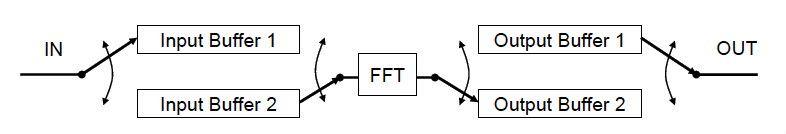
\includegraphics[width=\textwidth]{Segmentverarbeitung.png}
  \caption{Segmentverarbeitung mit Wechselbuffer, Quelle: Purat, S. 17}
  \label{fig:BufferRequire}
\end{figure}

Dabei sollte auf beiden Seiten ein zweiteiliger Buffer implementiert werden, dies hat den Hintergrund, dass die FFT immer über eine bestimmt Anzahl von Werten angewendet wird.
Da die FFT aber Länger als \begin{math}\frac{1}{Abtast} = \frac{1}{48 kHz}\end{math} dauert und der Buffer nicht geändert werden darf solange die FFT bearbeitet wird muss hier mit einem Arbeitsbuffer und einem temporären Buffer gearbeitet werden. Dies wurde in dem Source-Code \autoref{code:isrBuffer} implementiert.
\lstinputlisting[title=Routine zum aufnehmen der Samples und umschalten der Buffer]{isr.c}\label{code:isrBuffer}

Zu erst wurden in Zeile 20 - 22 benötigten Pointer und Arrays zum umschalten deklariert.
In Zeile 36 - 49 werden je nach dem zuletzt verwendetet Buffer die Bufferadressen geändert, dies geschieht immer bei der Aufnahme des ersten Samples.
Zeile 53 und 55 dienen zum Einlesen des Signals und zum Ausgeben des Spektrums. Sobald genug Samples aufgenommen wurden wird in Zeile 59 - 62 ein Trigger gesetzt und eine Flag für die FFT gesetzt.

Im weiteren musste eine Routine zur Berechnung des Betragsspektrums erstellt werden. Diese sollte in Assembler geschrieben werden. Die Umsetzung ist in dem Source-Code \autoref{code:abs2_spec} zu sehen.
\lstinputlisting[title=Routine zum berechnen des Betragsspektrums]{tools.asm}\label{code:abs2_spec}

Im ersten Teil, von Zeile 16 - 18 mussten die Eingangsparameter übernommen werden. Diese waren zum einen  die Pointer vom Komplexen Spektrum und zum Betragsspektrum, welches nun berechnet werden sollte und die Ordnung der FFT.
Zur Skalierung wurde in Zeile 20 ein Schiebe Faktor von 10 festgelegt.
In Zeile 24 wurde der erste Wert zu Berechnung eingelesen. Zeile 26 ist der beginn der Hardware Schleife diese soll der Ordnung entsprechend durchlaufen werden. Zeile 28 - 29 bilden die Betragsfunktion der komplexen Rechnung ab, diese ist in der Gleichung \ref{eq:komplBetrag} zu sehen.
\begin{equation}
\label{eq:komplBetrag}
	\mid z \mid = \sqrt{a^2 + b^2}
\end{equation} 
In Zeile 28 wird das Quadrat eines Wertes gebildet gebildet und der nächste Wert eingelesen. 
Zeile 29 realisiert die Bildung des zweiten quadrates, sowie die Addition beider Werte und das Auslesen des nächsten Werten. Die Skalierung in Zeile 30 wurde bereits in Zeile 20 vorbereitet.
Am Ende der Loop wird der berechnete Wert ausgegeben und der Pointer um eine Stelle erhöht. 
\section{Auswertung}\label{AFFToF}
\subsection*{Leck-Effekt}
Bevor zu Analyse der FFT kommen wollen wir noch über den Leck-Effekt reden, welcher uns im Laufe der Bearbeitung der Aufgaben aufgefallen ist. In \cref{fig:oLeckEffekt} ist zu sehen wie der schwarze Graph eine SI-Funktion darstellt, dies entsteht durch das Tiefpass-Verhalten des Ausganges. Unser Spektrum sollte im Idealfall genau ein Impuls sein, dadurch ist das Ausgangssignal die Impulsantwort des Ausganges, welches eine SI-Funktion ist. 
\begin{figure}[H]
	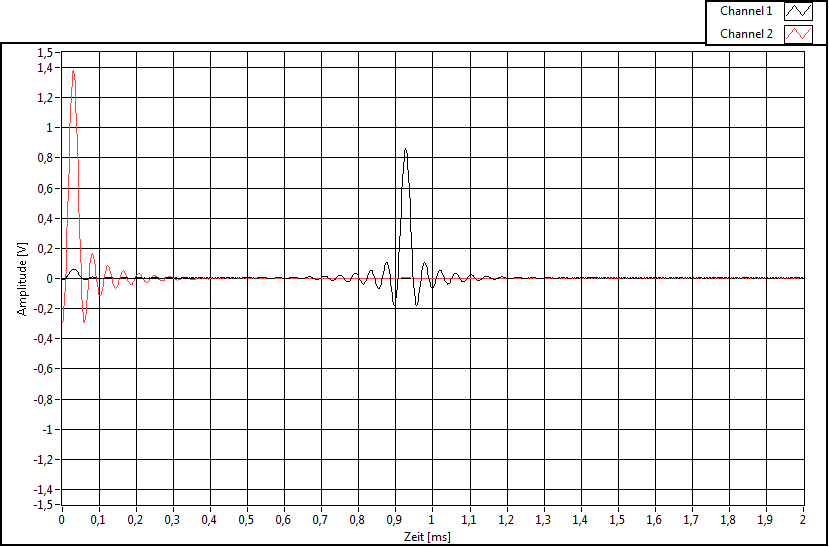
\includegraphics[width=\textwidth]{keinLeckeffekt505Hz.png}
  \caption{Ausgangssignal(505 Hz) ohne Leck-Effekt}
  \label{fig:oLeckEffekt}
\end{figure}
In \cref{fig:mLeckEffekt} ist zu sehen, dass das Ausgangssignal keine SI-Funktion darstellt.

\begin{figure}[H]
	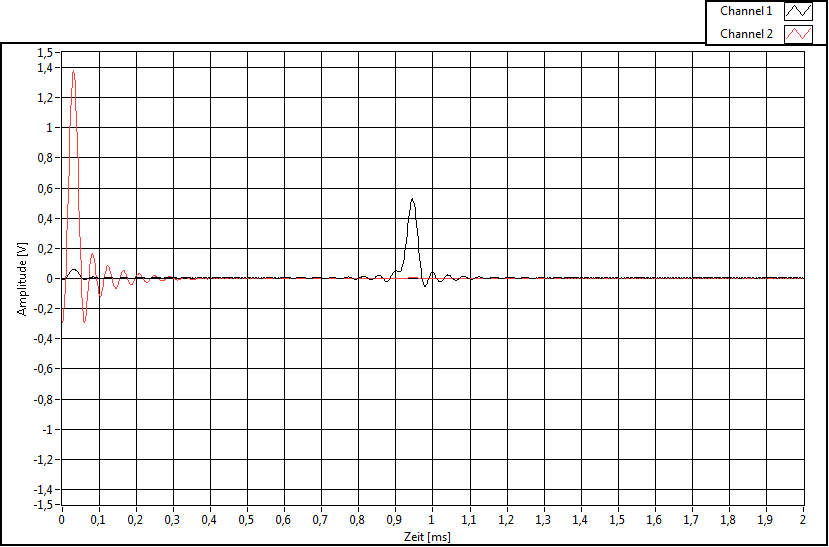
\includegraphics[width=\textwidth]{Leckeffekt511Hz.png}
  \caption{Ausgangssignal(511 Hz) mit Leck-Effekt}
  \label{fig:mLeckEffekt}
\end{figure}
Der Leck-Effekt tritt bei Spektralanalysen auf, welche keinen unendlichen langen Beobachtungszeitraum besitzen, also praktisch bei allen. Durch den Leck-Effekt werden Frequenzen um die eigentliche Frequenz berechnet, welche nicht vorhanden sind. Dieser Effekt kann verhindert werden, indem eine Abtastfrequenz gewählt wird, welche dem ganzzahligen Vielfachen der Signalfrequenz entspricht. Natürlich sind hierbei Ungenauigkeiten zu beachten weshalb die von uns gewählten Frequenzen nicht berechnet wurden, sondern durch ausprobieren ermittelt wurden. 
\newpage
Mit diesem Wissen können wir nun die Analyse der DTMF Frequenzen beginnen. Als Frequenzen haben wir die ersten beiden Zeilenfrequenzen gewählt, diese sind 697 Hz und 770 Hz.
Zur besseren Darstellung, haben wir jeweils ein Bild mit passender Achseneinteilung ein Detailbild genommen. Die Achseneinteilung wurde so gewählt das ein Kästchen 1,2 kHz entspricht, somit ist es möglich zu bewerten ob unsere FFT ordentlich arbeitet. In \cref{fig:Spekt697} ist ein Impuls leicht über der Mitte des ersten Kästchens zu sehen. Dies bedeutet, dass wir davon ausgehen können das es sich hierbei um die 697 Hz handeln kann.
\begin{figure}[H]
	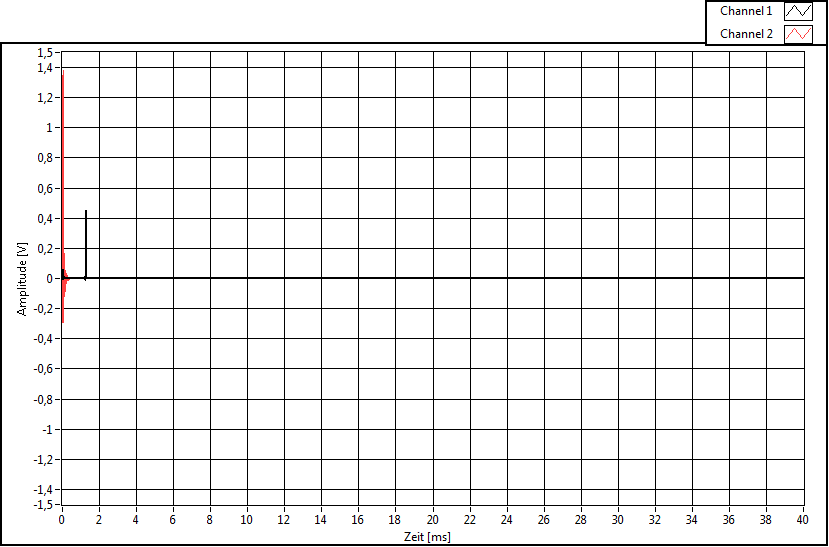
\includegraphics[width=\textwidth]{Spektrum697Hz.png}
  \caption{Ausgangsspektrum bei einem 697 Hz Eingangssignal}
  \label{fig:Spekt697}
\end{figure}

\cref{fig:Spekt697Close} zeigt eine Nahaufnahme des Spektrums, dort ist der Leck-Effekt deutlich zu sehen. Außerdem ist nun zu sehen das sich der Impuls sehr nahe an den 697 Hz bewegt, denn \begin{math} \frac{1,26ms}{2ms} * 1,2 kHz = 0,762 kHz \end{math}. Dies liegt augenscheinlich erstmal näher bei 770 Hz allerdings werden wir gleich sehen, dass auch das Spektrum des zweiten Signals leicht nach hinten verschoben ist. 
\begin{figure}[H]
	\includegraphics[width=\textwidth]{Spektrum697CloseHz.png}
  \caption{Ausgangsspektrum bei einem 697 Hz Eingangssignal}
  \label{fig:Spekt697Close}
\end{figure}

\cref{fig:Spekt770} zeigt ein ähnliches Bild wie \cref{fig:Spekt697} und weißt keine Besonderheiten auf.
\begin{figure}[H]
	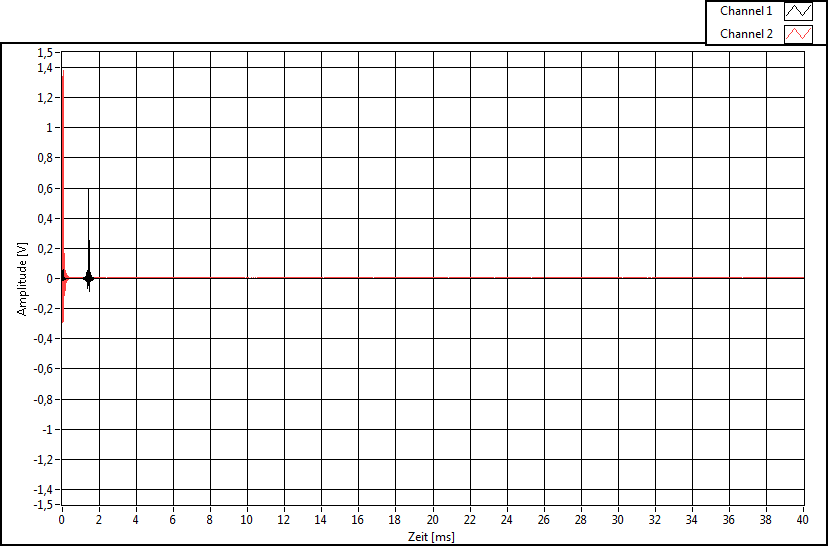
\includegraphics[width=\textwidth]{Spektrum770Hz.png}
  \caption{Ausgangsspektrum bei einem 770 Hz Eingangssignal}
  \label{fig:Spekt770}
\end{figure}

In \cref{fig:Spekt770Close} ist zu sehen das bei 770 Hz kein oder nur ein sehr schwacher Leck-Effekt auftritt. Außerdem ist zu sehen, dass dieses Spektrum ebenfalls weiter als erwartet nach rechts verschoben ist. An dieser Stelle wäre das Spektrum eines 840 Hz Signals zu erwarten, \begin{math} \frac{1,4ms}{2ms} * 1,2 kHz = 0,84 kHz \end{math}
\begin{figure}[H]
	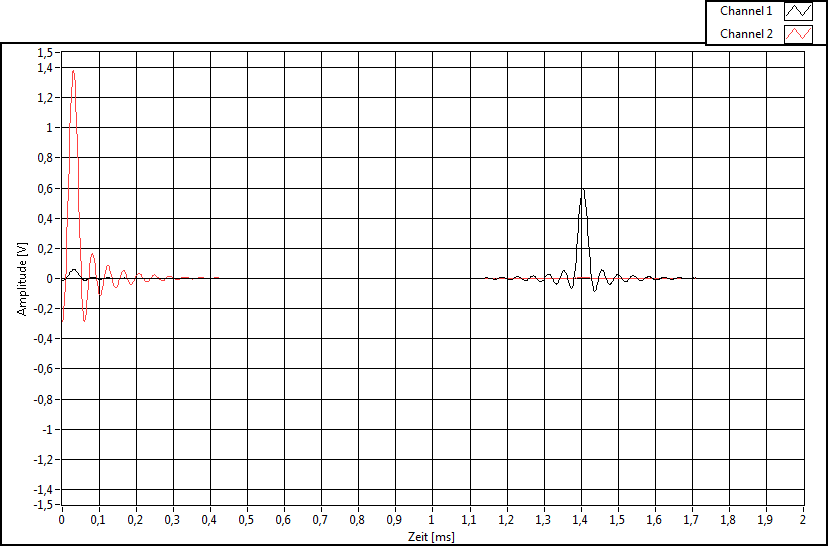
\includegraphics[width=\textwidth]{Spektrum770HzClose.png}
  \caption{Ausgangsspektrum bei einem 770 Hz Eingangssignal}
  \label{fig:Spekt770Close}
\end{figure}